\documentclass{standalone}
% This file was created with tikzplotlib v0.9.15.

\usepackage{siunitx}
\usepackage{pgfplots}
% and optionally (as of Pgfplots 1.3):
\pgfplotsset{compat=newest}
\pgfplotsset{plot coordinates/math parser=false}
\newlength\figureheight
\newlength\figurewidth

\newcommand{\Set}[1]{\mathcal{#1}}
\newcommand{\Vector}[1]{\bm{\MakeLowercase{#1}}}
\newcommand{\Operator}[1]{\bm{\MakeUppercase{#1}}}
%%%%%%%%%%
\DeclareMathAlphabet{\mathsfbr}{OT1}{cmss}{m}{n}%for math sans serif (cmss)
\SetMathAlphabet{\mathsfbr}{bold}{OT1}{cmss}{bx}{n}%for math sans serif (cmss)
\DeclareRobustCommand{\msf}[1]{%
  \ifcat\noexpand#1\relax\msfgreek{#1}\else\mathsfbr{#1}\fi%for math sans serif (cmss)
}
\DeclareFontEncoding{LGR}{}{} % or load \usepackage{textgreek}
\DeclareSymbolFont{sfgreek}{LGR}{cmss}{m}{n}
\SetSymbolFont{sfgreek}{bold}{LGR}{cmss}{bx}{n}
\DeclareMathSymbol{\sXi}{\mathalpha}{sfgreek}{`X}
\DeclareMathSymbol{\sUpsilon}{\mathalpha}{sfgreek}{`U}

\begin{document}

% This file was created with tikzplotlib v0.9.15.
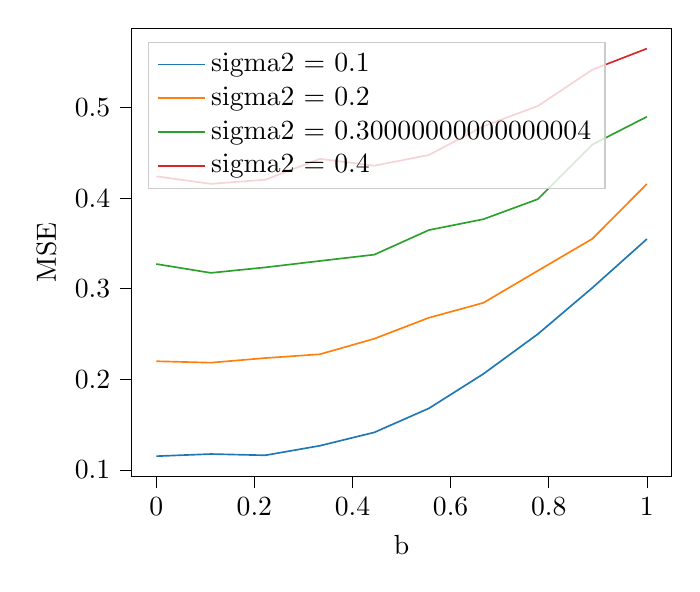
\begin{tikzpicture}

\definecolor{color0}{rgb}{0.12156862745098,0.466666666666667,0.705882352941177}
\definecolor{color1}{rgb}{1,0.498039215686275,0.0549019607843137}
\definecolor{color2}{rgb}{0.172549019607843,0.627450980392157,0.172549019607843}
\definecolor{color3}{rgb}{0.83921568627451,0.152941176470588,0.156862745098039}

\begin{axis}[
legend cell align={left},
legend style={
  fill opacity=0.8,
  draw opacity=1,
  text opacity=1,
  at={(0.03,0.97)},
  anchor=north west,
  draw=white!80!black
},
tick align=outside,
tick pos=left,
x grid style={white!69.0196078431373!black},
xlabel={b},
xmin=-0.05, xmax=1.05,
xtick style={color=black},
y grid style={white!69.0196078431373!black},
ylabel={MSE},
ymin=0.0925075, ymax=0.5877825,
ytick style={color=black}
]
\addplot [semithick, color0]
table {%
0 0.11502
0.111111111111111 0.117392
0.222222222222222 0.116006
0.333333333333333 0.126538
0.444444444444444 0.141316
0.555555555555556 0.16781
0.666666666666667 0.20589
0.777777777777778 0.249924
0.888888888888889 0.30105
1 0.354898
};
\addlegendentry{sigma2 = 0.1}
\addplot [semithick, color1]
table {%
0 0.219902
0.111111111111111 0.218308
0.222222222222222 0.223424
0.333333333333333 0.227606
0.444444444444444 0.244784
0.555555555555556 0.267936
0.666666666666667 0.2844
0.777777777777778 0.31989
0.888888888888889 0.355172
1 0.415776
};
\addlegendentry{sigma2 = 0.2}
\addplot [semithick, color2]
table {%
0 0.327306
0.111111111111111 0.317518
0.222222222222222 0.32359
0.333333333333333 0.33068
0.444444444444444 0.337656
0.555555555555556 0.3648
0.666666666666667 0.37679
0.777777777777778 0.398976
0.888888888888889 0.459256
1 0.489998
};
\addlegendentry{sigma2 = 0.30000000000000004}
\addplot [semithick, color3]
table {%
0 0.42416
0.111111111111111 0.415874
0.222222222222222 0.420442
0.333333333333333 0.443416
0.444444444444444 0.435928
0.555555555555556 0.447734
0.666666666666667 0.479462
0.777777777777778 0.50183
0.888888888888889 0.541948
1 0.56527
};
\addlegendentry{sigma2 = 0.4}
\end{axis}

\end{tikzpicture}

\end{document}